\chapter{जंतुओं की शरीर-योजनाएँ और ऊतक}\label{ch:b1:body-plans-tissues}

प्रयोगशाला की मेज़ पर चार जंतु: एक सेंटीमीटर लंबा एक हाइड्रा, एक केंचुआ,
एक क्रेफ़िश, एक मेंढक। आकार और स्वभाव के भेदों के नीचे वे मुट्ठी भर साझा
निर्णयों पर बने हैं --- शरीर का कोई आगा और पीछा है या नहीं, वह कोशिकाओं
की कितनी परतों से उगा, आँत के चारों ओर कोई गुहा है या नहीं, शरीर दोहराए
गए खंडों का बना है या नहीं, कंकाल कहाँ है --- और इनमें से हर एक उन्हीं
चार प्रकार के \omterm{def:b1:body-plans-tissues:tissue}{ऊतकों} से बना है। यह अध्याय जंतुओं की \omterm{def:b1:mammal-organization:bodyplan}{शरीर-योजनाएँ} और उन्हें
बनाने वाले \omterm{def:b1:body-plans-tissues:tissue}{ऊतक} प्रस्तुत करता है, और वहीं समाप्त होता है जहाँ पिछले
अध्याय छूटे थे: किसी स्तनधारी की \omterm{prop:b1:body-plans-tissues:gutwall}{आँत की भित्ति} पर, जिसे एक \omterm{def:b1:mammal-organization:organ}{अंग} में जुड़े
\omterm{def:b1:body-plans-tissues:tissue}{ऊतकों} के रूप में देखा जाता है।

\section{शरीर-योजनाएँ}

\begin{definition}[सममिति और शीर्षीभवन]\label{def:b1:body-plans-tissues:symmetry}
किसी जंतु में \emph{अरीय सममिति}\index{अरीय सममिति} तब होती है जब उसका
शरीर किसी केंद्रीय अक्ष के चारों ओर सजा हो और उसमें बायाँ-दायाँ न हो,
जैसे हाइड्रा या जेलीफ़िश में: वह अपने पर्यावरण से सब ओर से बराबर मिलता
है, और प्रायः स्थिर रहता है या बहता है। उसमें \emph{द्विपार्श्व
सममिति}\index{द्विपार्श्व सममिति} तब होती है जब कोई एक तल उसे दर्पण-आधों
में बाँटता हो, और इस तरह एक अगला (अग्र) और पिछला (पश्च) सिरा, तथा एक
पीठ (पृष्ठ) और एक पेट (अधर) परिभाषित करता हो: यह उस जंतु की योजना है जो
सिर आगे करके चलता है और जिसकी ज्ञानेंद्रियाँ तथा तंत्रिका केंद्र आगे
जमा होते हैं (\omterm{def:b1:mammal-organization:bodyplan}{शीर्षीभवन})।
\end{definition}

\begin{definition}[जनन स्तर, देहगुहाएँ]\label{def:b1:body-plans-tissues:layers}
किसी जंतु का भ्रूण कोशिकाओं की दो या तीन परतें बनाता है, यानी
\emph{जनन स्तर}\index{जनन स्तर}, जिनसे सारे \omterm{def:b1:body-plans-tissues:tissue}{ऊतक} निकलते हैं: बाहरी
\emph{बाह्यचर्म}\index{बाह्यचर्म} (त्वचा, तंत्रिका तंत्र), भीतरी
\emph{अंतश्चर्म}\index{अंतश्चर्म} (आँत और उसकी उपजों का अस्तर) और,
स्पंजों तथा निडारियों को छोड़कर सबमें, एक बीच का
\emph{मध्यचर्म}\index{मध्यचर्म} (पेशी, कंकाल, \omterm{def:b1:body-plans-tissues:connective}{संयोजी ऊतक}, रक्त, गुर्दे,
जनद)। निडारी \emph{द्विजनस्तरी} हैं, बाक़ी \emph{त्रिजनस्तरी}।
त्रिजनस्तरी जंतुओं में मध्यचर्म या तो आँत और देह-भित्ति के बीच की जगह
भर देता है (\emph{अगुहीय}: चपटे कृमि), या उनके बीच एक गुहा छोड़ता है:
जब गुहा पूरी तरह मध्यचर्म से अस्तरित हो तो वह
\emph{देहगुहा}\index{देहगुहा} है (एनेलिड, मोलस्क, संधिपाद, शूलचर्मी,
कशेरुकी)। देहगुहा आँत को उसके अपने कक्ष में लटकाती है, उसे देह-भित्ति से
स्वतंत्र चलने देती है, और कोमल शरीर वालों को एक \omterm{def:b1:body-plans-tissues:segments}{द्रवस्थैतिक कंकाल} देती
है।
\end{definition}

\begin{omfigure}
\begin{tikzpicture}[font=\footnotesize, line cap=round]
  \node[font=\small, anchor=south] at (1.4,2.75) {अगुहीय (चपटा कृमि)};
  \node[font=\small, anchor=south] at (6.6,2.75) {देहगुहीय (एनेलिड, कशेरुकी)};
  % acoelomate: body wall ectoderm, solid mesoderm, gut endoderm
  \draw[thick, fill=omDef!25] (1.4,1.3) ellipse (1.35 and 1.25);
  \fill[omProp!35] (1.4,1.3) ellipse (1.15 and 1.05);
  \draw[thick, fill=omExo!30] (1.4,1.3) ellipse (0.4 and 0.35);
  \node at (1.4,1.3) {आँत};
  \node at (1.4,0.62) {मध्यचर्म};
  % coelomate: body wall, coelom, gut with mesoderm layer
  \draw[thick, fill=omDef!25] (6.6,1.3) ellipse (1.35 and 1.25);
  \fill[omProp!35] (6.6,1.3) ellipse (1.15 and 1.05);
  \fill[white] (6.6,1.3) ellipse (0.95 and 0.85);
  \draw[thick, fill=omProp!35] (6.6,1.3) ellipse (0.55 and 0.5);
  \draw[thick, fill=omExo!30] (6.6,1.3) ellipse (0.4 and 0.35);
  \node at (6.6,1.3) {आँत};
  \node at (6.6,0.62) {देहगुहा};
  % legend
  \fill[omDef!25] (8.9,2.2) rectangle +(0.35,0.25); \node[anchor=west] at (9.3,2.32) {बाह्यचर्म};
  \fill[omProp!35] (8.9,1.7) rectangle +(0.35,0.25); \node[anchor=west] at (9.3,1.82) {मध्यचर्म};
  \fill[omExo!30] (8.9,1.2) rectangle +(0.35,0.25); \node[anchor=west] at (9.3,1.32) {अंतश्चर्म};
  \draw (8.9,0.7) rectangle +(0.35,0.25); \node[anchor=west] at (9.3,0.82) {देहगुहा (गुहा)};
\end{tikzpicture}

{\small दो त्रिजनस्तरी शरीर-योजनाओं की अनुप्रस्थ काटें। अगुहीय में
\omterm{def:b1:body-plans-tissues:layers}{मध्यचर्म} देह-भित्ति और आँत के बीच की जगह भर देता है; देहगुहीय में
\omterm{def:b1:body-plans-tissues:layers}{मध्यचर्म} से अस्तरित एक गुहा उन्हें अलग करती है, ताकि आँत स्वतंत्र लटके
और गुहा का द्रव कंकाल का काम कर सके।}
\end{omfigure}

\begin{definition}[अग्रमुखी और पश्चमुखी]\label{def:b1:body-plans-tissues:proto}
देहगुहीय जंतुओं में भ्रूणीय आँत के पहले छिद्र की नियति दो बड़ी वंशरेखाएँ
अलग करती है: \emph{अग्रमुखियों}\index{अग्रमुखी} में (एनेलिड, मोलस्क,
संधिपाद) वह मुँह बनता है, \omterm{def:b1:body-plans-tissues:layers}{देहगुहा} \omterm{def:b1:body-plans-tissues:layers}{मध्यचर्म} के फटने से बनती है, और अंडे
के आरंभिक विदलन सर्पिल होते हैं तथा उनकी नियति जल्दी तय हो जाती है;
\emph{पश्चमुखियों}\index{पश्चमुखी} में (शूलचर्मी, कशेरुकी) वह गुदा बनता
है, \omterm{def:b1:body-plans-tissues:layers}{देहगुहा} आँत की थैलियाँ निकलने से बनती है, और आरंभिक कोशिकाएँ अपनी
नियति में लचीली बनी रहती हैं।
\end{definition}

\begin{definition}[खंडीभवन, कंकाल]\label{def:b1:body-plans-tissues:segments}
कोई शरीर \emph{खंडित}\index{खंडीभवन} तब होता है जब वह अपने अक्ष के
सहारे दोहराई गई इकाइयों से बना हो (केंचुए के छल्ले, क्रेफ़िश के खंड,
मछली के कशेरुक और पेशी-गुटके), और हर इकाई के पास अपनी पेशियाँ, अपनी
तंत्रिकाएँ और प्रायः अपने उपांग हों। खंड एक जैसे हो सकते हैं या क्षेत्रों
में विशिष्ट (सिर, वक्ष, उदर)। \emph{कंकाल}\index{कंकाल}, जिसके विरुद्ध
पेशियाँ खिंचती हैं, या तो \emph{द्रवस्थैतिक}\index{द्रवस्थैतिक कंकाल}
होता है (किसी \omterm{def:b1:body-plans-tissues:layers}{देहगुहा} में दाब के नीचे कोई द्रव, जैसे केंचुए में), या
\emph{बाह्यकंकाल}\index{बाह्यकंकाल} (शरीर के बाहर की कोई कठोर \omterm{def:b1:flowering-plant-organization:tissues}{उपचर्म},
संधियुक्त, जो बढ़ने के लिए निर्मोचित होती है, जैसे संधिपादों में), या
\emph{अंतःकंकाल}\index{अंतःकंकाल} (शरीर के भीतर की उपास्थि या हड्डी, जो
उसके साथ बढ़ती है, जैसे कशेरुकियों में)।
\end{definition}

\begin{omfigure}
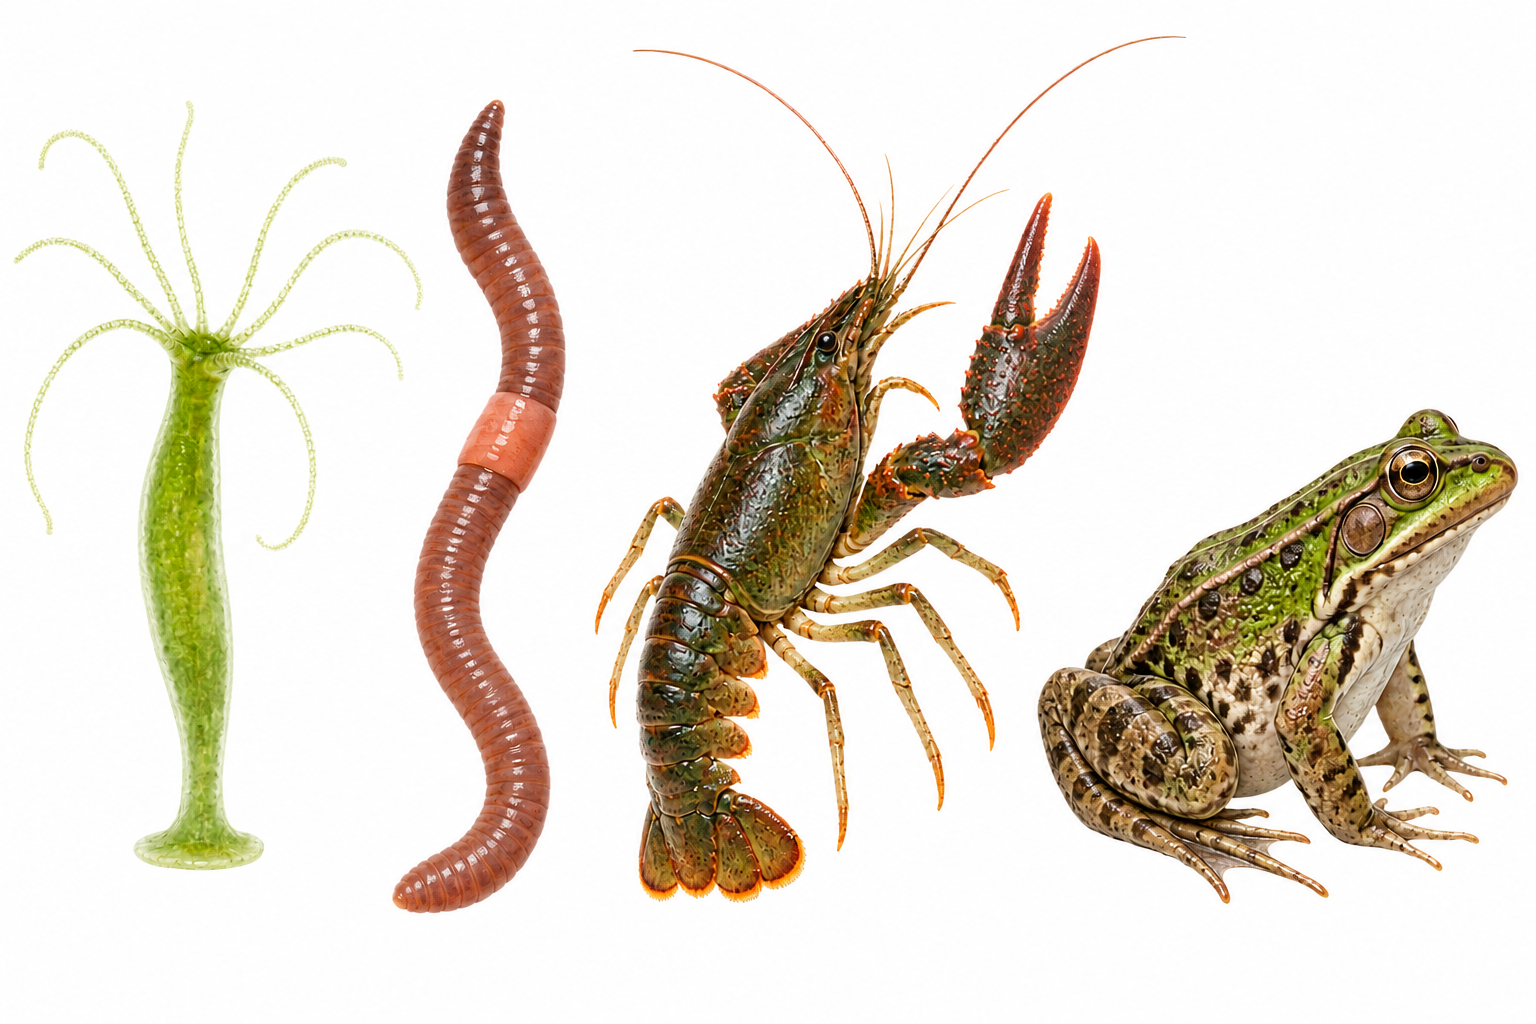
\includegraphics[width=0.78\linewidth]{images/book3/ai/b3-04-body-plans.png}

{\small चार \omterm{def:b1:mammal-organization:bodyplan}{शरीर-योजनाएँ}। एक हाइड्रा (अरीय, दो परतें, \omterm{def:b1:body-plans-tissues:layers}{देहगुहा} नहीं), एक
केंचुआ (द्विपार्श्व, देहगुहीय, \omterm{def:b1:body-plans-tissues:segments}{खंडित}, \omterm{def:b1:body-plans-tissues:segments}{द्रवस्थैतिक कंकाल}), एक क्रेफ़िश
(विशिष्ट क्षेत्रों सहित \omterm{def:b1:body-plans-tissues:segments}{खंडित}, संधियुक्त \omterm{def:b1:body-plans-tissues:segments}{बाह्यकंकाल}) और एक मेंढक
(\omterm{def:b1:body-plans-tissues:proto}{पश्चमुखी}, हड्डी का \omterm{def:b1:body-plans-tissues:segments}{अंतःकंकाल})।}
\end{omfigure}

\begin{proposition}[चार योजनाओं की तुलना]\label{prop:b1:body-plans-tissues:four}
\begin{center}
\small
\begin{tabular}{lllll}
\hline
 & हाइड्रा & केंचुआ & क्रेफ़िश & मेंढक \\
\hline
सममिति & अरीय & द्विपार्श्व & द्विपार्श्व & द्विपार्श्व \\
\omterm{def:b1:body-plans-tissues:layers}{जनन स्तर} & 2 & 3 & 3 & 3 \\
\omterm{def:b1:body-plans-tissues:layers}{देहगुहा} & नहीं & हाँ & घटी हुई & हाँ \\
वंशरेखा & --- & \omterm{def:b1:body-plans-tissues:proto}{अग्रमुखी} & \omterm{def:b1:body-plans-tissues:proto}{अग्रमुखी} & \omterm{def:b1:body-plans-tissues:proto}{पश्चमुखी} \\
खंड & नहीं & एक जैसे & विशिष्ट & कशेरुक, पेशी-गुटके \\
कंकाल & द्रवस्थैतिक & द्रवस्थैतिक & \omterm{def:b1:body-plans-tissues:segments}{बाह्यकंकाल} & \omterm{def:b1:body-plans-tissues:segments}{अंतःकंकाल} \\
आँत & एक छिद्र & मुँह से गुदा & मुँह से गुदा & मुँह से गुदा \\
परिसंचरण & नहीं & बंद & खुला & बंद, हृदय \\
तंत्रिका तंत्र & जाल & अधर रज्जु & अधर रज्जु & पृष्ठ रज्जु \\
\hline
\end{tabular}
\end{center}
ये योजनाएँ किसी सीढ़ी के डंडे नहीं हैं: हर एक जंतु होने का एक पूर्ण और
सफल ढंग है, और क्रेफ़िश तथा मेंढक एक-दूसरे के समकालीन हैं, पूर्वज नहीं।
\end{proposition}

\begin{example}[किसी जंतु को उसकी योजना से पढ़ना]\label{ex:b1:body-plans-tissues:reading}
कोई जंतु जिसका एक शिरोभाग है, एक आरपार आँत है, एक जैसे छल्लों का शरीर
है और कोई कठोर भाग नहीं: यह देहगुहीय \omterm{def:b1:body-plans-tissues:proto}{अग्रमुखी} है जो \omterm{def:b1:body-plans-tissues:segments}{द्रवस्थैतिक कंकाल} से
चलता है, और जिसके हर खंड का देहगुहा-द्रव बारी-बारी से वर्तुल तथा
अनुदैर्घ्य पेशियों से दाबित होता है --- यानी बिल खोदता कोई केंचुआ। कोई
जंतु जिसकी \omterm{def:b1:flowering-plant-organization:tissues}{उपचर्म} संधियुक्त है और खंड विशिष्ट: कोई संधिपाद, जिसकी वृद्धि
को निर्मोचनों से गुज़रना पड़ता है। कशेरुकों के किसी पृष्ठ अक्ष के चारों
ओर द्विपार्श्व, \omterm{def:b1:body-plans-tissues:segments}{खंडित} पेशी-गुटके: कोई कशेरुकी, जिसका \omterm{def:b1:body-plans-tissues:segments}{अंतःकंकाल} लगातार
बढ़ता है।
\end{example}

\section{ऊतकों के चार प्रकार}

\begin{definition}[ऊतक]\label{def:b1:body-plans-tissues:tissue}
\emph{ऊतक}\index{ऊतक} समान संरचना और उद्गम की कोशिकाओं का वह समूह है
जो, उनके बनाए बाह्यकोशिकीय पदार्थ के साथ, किसी साझा कार्य के लिए संगठित
हो। जंतु-ऊतक चार प्रकारों में आते हैं: \omterm{def:b1:body-plans-tissues:epithelium}{उपकला}, संयोजी, पेशी, तंत्रिका। हर
\omterm{def:b1:mammal-organization:organ}{अंग} इनमें से कम से कम दो का संयोजन है।
\end{definition}

\begin{definition}[उपकला ऊतक]\label{def:b1:body-plans-tissues:epithelium}
\emph{उपकला}\index{उपकला} पास-पास जमी कोशिकाओं की वह चादर है जो किसी
सतह को ढकती है या किसी गुहा को अस्तरित करती है, और जो \omterm{def:b1:body-plans-tissues:connective}{बाह्यकोशिकीय
आधात्री} की एक पतली परत, यानी \emph{आधार पटलिका}\index{आधार पटलिका}, पर
टिकी होती है। उसकी कोशिकाएँ \emph{ध्रुवित}\index{कोशिका ध्रुवता} होती
हैं: शीर्ष फलक बाहर या अवकाशिका की ओर देखता है, आधार फलक पटलिका की ओर,
और दोनों अलग-अलग प्रोटीन धारण करते हैं। वे \emph{कोशिका
संधियों}\index{कोशिका संधि} से जुड़ी होती हैं: शीर्ष के पास
\emph{दृढ़ संधियाँ}, जो कोशिकाओं के बीच की जगह इस तरह सील करती हैं कि
कोशिकाओं से होकर ही कुछ चादर पार कर सके; \emph{आसंजी संधियाँ} और
\emph{डेस्मोसोम}, जो कोशिकाओं को यांत्रिक रूप से बाँधते हैं; और
\emph{रिक्ति संधियाँ}, यानी ऐसे चैनल जो आयनों और छोटे अणुओं को कोशिका से
कोशिका तक जाने देते हैं। उपकलाएँ परतों की संख्या (सरल, स्तरित) और
कोशिकाओं की आकृति (शल्की, घनाकार, स्तंभाकार) से वर्गीकृत होती हैं, और
इनमें ग्रंथियाँ भी आती हैं, जो स्राव में विशिष्ट उपकला कोशिकाएँ हैं। वे
ढकती हैं, रक्षा करती हैं, अवशोषित करती हैं और स्रावित करती हैं।
\end{definition}

\begin{omfigure}
\begin{tikzpicture}[font=\footnotesize, line cap=round]
  % three columnar cells
  \foreach \x in {0,1.6,3.2} {
    \draw[thick, fill=omDef!10] (\x,0) rectangle (\x+1.5,3.2);
    \fill[omDef!60] (\x+0.75,0.9) ellipse (0.32 and 0.42);
    % microvilli
    \foreach \m in {0.15,0.35,0.55,0.75,0.95,1.15,1.35} \draw[omDef!70!black, thick] (\x+\m,3.2) -- (\x+\m,3.5);
  }
  % junctions between cell 1-2 and 2-3
  \foreach \x in {1.55,3.15} {
    \draw[very thick, omThm] (\x-0.05,2.9) -- (\x+0.1,2.9);
    \draw[very thick, omProp] (\x-0.05,2.5) -- (\x+0.1,2.5);
    \draw[very thick, omProp] (\x-0.05,1.9) -- (\x+0.1,1.9);
    \draw[very thick, omExo] (\x-0.05,1.2) -- (\x+0.1,1.2);
  }
  % basal lamina
  \draw[very thick, gray!70] (-0.2,-0.05) -- (4.9,-0.05);
  \fill[pattern=north east lines, pattern color=gray!50] (-0.2,-0.6) rectangle (4.9,-0.1);
  % labels
  \node[anchor=south] at (2.4,3.55) {शीर्ष फलक: सूक्ष्मांकुर, अवकाशिका की ओर};
  \node[anchor=west, omThm] at (5.1,2.9) {दृढ़ संधि: दरार सील करती है};
  \node[anchor=west, omProp] at (5.1,2.5) {आसंजी संधि: ऐक्टिन पट्टी};
  \node[anchor=west, omProp] at (5.1,1.9) {डेस्मोसोम: यांत्रिक रिवेट};
  \node[anchor=west, omExo] at (5.1,1.2) {रिक्ति संधि: कोशिका-से-कोशिका चैनल};
  \node[anchor=west, gray!80!black] at (5.1,-0.05) {आधार पटलिका};
  \node[anchor=west, gray!80!black] at (5.1,-0.45) {नीचे संयोजी ऊतक};
  \node[anchor=east] at (-0.3,0.9) {केंद्रक};
\end{tikzpicture}

{\small एक सरल स्तंभाकार \omterm{def:b1:body-plans-tissues:epithelium}{उपकला}, जैसी आँत में होती है। हर कोशिका का एक
शीर्ष फलक है जो सूक्ष्मांकुर धारण करता है और एक आधार फलक जो \omterm{def:b1:body-plans-tissues:epithelium}{आधार पटलिका}
पर है; पड़ोसी दृढ़ संधियों से सील हैं, आसंजी संधियों तथा डेस्मोसोमों से
बँधे हैं, और रिक्ति संधियों से जुड़े हैं।}
\end{omfigure}

\begin{definition}[संयोजी ऊतक]\label{def:b1:body-plans-tissues:connective}
\emph{संयोजी ऊतक}\index{संयोजी ऊतक} बिखरी कोशिकाओं से बना है जो अपनी ही
स्रावित की हुई प्रचुर \emph{बाह्यकोशिकीय आधात्री}\index{बाह्यकोशिकीय आधात्री} में रहती हैं: प्रोटीन तंतु --- \emph{कोलैजन}\index{कोलैजन}
(तन्य सामर्थ्य; किसी स्तनधारी के सारे प्रोटीन का एक-चौथाई),
\emph{इलैस्टिन}\index{इलैस्टिन} (प्रत्यानयन) --- जो बहुशर्कराओं के किसी
जलयोजित \emph{भरण पदार्थ} में धँसे होते हैं। अनुपात ही उसके प्रकार तय
करते हैं: \omterm{def:b1:body-plans-tissues:epithelium}{उपकलाओं} के नीचे और \omterm{def:b1:mammal-organization:organ}{अंगों} के चारों ओर ढीला संयोजी \omterm{def:b1:body-plans-tissues:tissue}{ऊतक}
(तंतुकोरक, थोड़े तंतु, बहुत भरण पदार्थ); कंडराओं और स्नायुओं का सघन
संयोजी \omterm{def:b1:body-plans-tissues:tissue}{ऊतक} (समांतर कोलैजन); वसा \omterm{def:b1:body-plans-tissues:tissue}{ऊतक} (वसा संचित करती कोशिकाएँ); उपास्थि
(कोलैजन और बहुशर्कराओं का एक दृढ़ जेल, बिना वाहिकाओं के); हड्डी (कैल्सियम
फ़ॉस्फ़ेट से खनिजित कोलैजन, गुहाओं में जीवित कोशिकाएँ, वाहिकाएँ); और
रक्त, जिसकी आधात्री प्लाज़्मा है। यह बाँधता है, आधार देता है, संचित करता
है, ढोता है और रक्षा करता है।
\end{definition}

\begin{definition}[पेशी ऊतक]\label{def:b1:body-plans-tissues:muscle}
\emph{पेशी ऊतक}\index{पेशी ऊतक} लंबी कोशिकाओं से बना है जो संकुचनशील
प्रोटीन तंतुकों (ऐक्टिन और मायोसिन) से भरी होती हैं। तीन प्रकार:
\emph{कंकाल पेशी}, जो लंबे बहुकेंद्रकी तंतुओं की है, जिनमें अनुप्रस्थ
धारियाँ दिखती हैं, जो कंकाल से जुड़ी हैं और ऐच्छिक नियंत्रण में हैं;
\emph{हृदय पेशी}, जो शाखित धारीदार कोशिकाओं की है जो सिरे से सिरे तक ऐसी
संधियों से जुड़ी हैं जो धड़कन कोशिका से कोशिका तक पहुँचाती हैं, और जो
अपनी ही लय पर संकुचित होती है; और \emph{चिकनी पेशी}, जो खोखले \omterm{def:b1:mammal-organization:organ}{अंगों}
(आँत, वाहिकाएँ, गर्भाशय) की भित्तियों में तर्कु-आकार की बिना धारी वाली
कोशिकाओं की है, और जो धीरे तथा अनैच्छिक रूप से संकुचित होती है। संकुचन की
क्रियाविधि वर्ष 2 के खंड में दी गई है।
\end{definition}

\begin{definition}[तंत्रिका ऊतक]\label{def:b1:body-plans-tissues:nervous}
\emph{तंत्रिका ऊतक}\index{तंत्रिका ऊतक} \emph{न्यूरॉनों}\index{न्यूरॉन}
से बना है, यानी ऐसी कोशिकाओं से जिनका एक काय और लंबे विस्तार हैं
(संकेत ग्रहण करती द्रुमिकाएँ, और उन्हें ले जाता एक अक्षतंतु), जो विद्युत
संकेतों का चालन करती हैं और उन्हें तंत्रिका-संधियों पर दूसरी कोशिकाओं तक
पहुँचाती हैं, तथा \emph{ग्लियल कोशिकाओं}\index{ग्लियल कोशिका} से, जो
कई गुना अधिक संख्या में हैं और न्यूरॉनों को आधार देती हैं, कुचालक करती
हैं और पोषती हैं। यह भाँपता है, समाकलित करता है और आदेश देता है।
\end{definition}

\begin{omfigure}
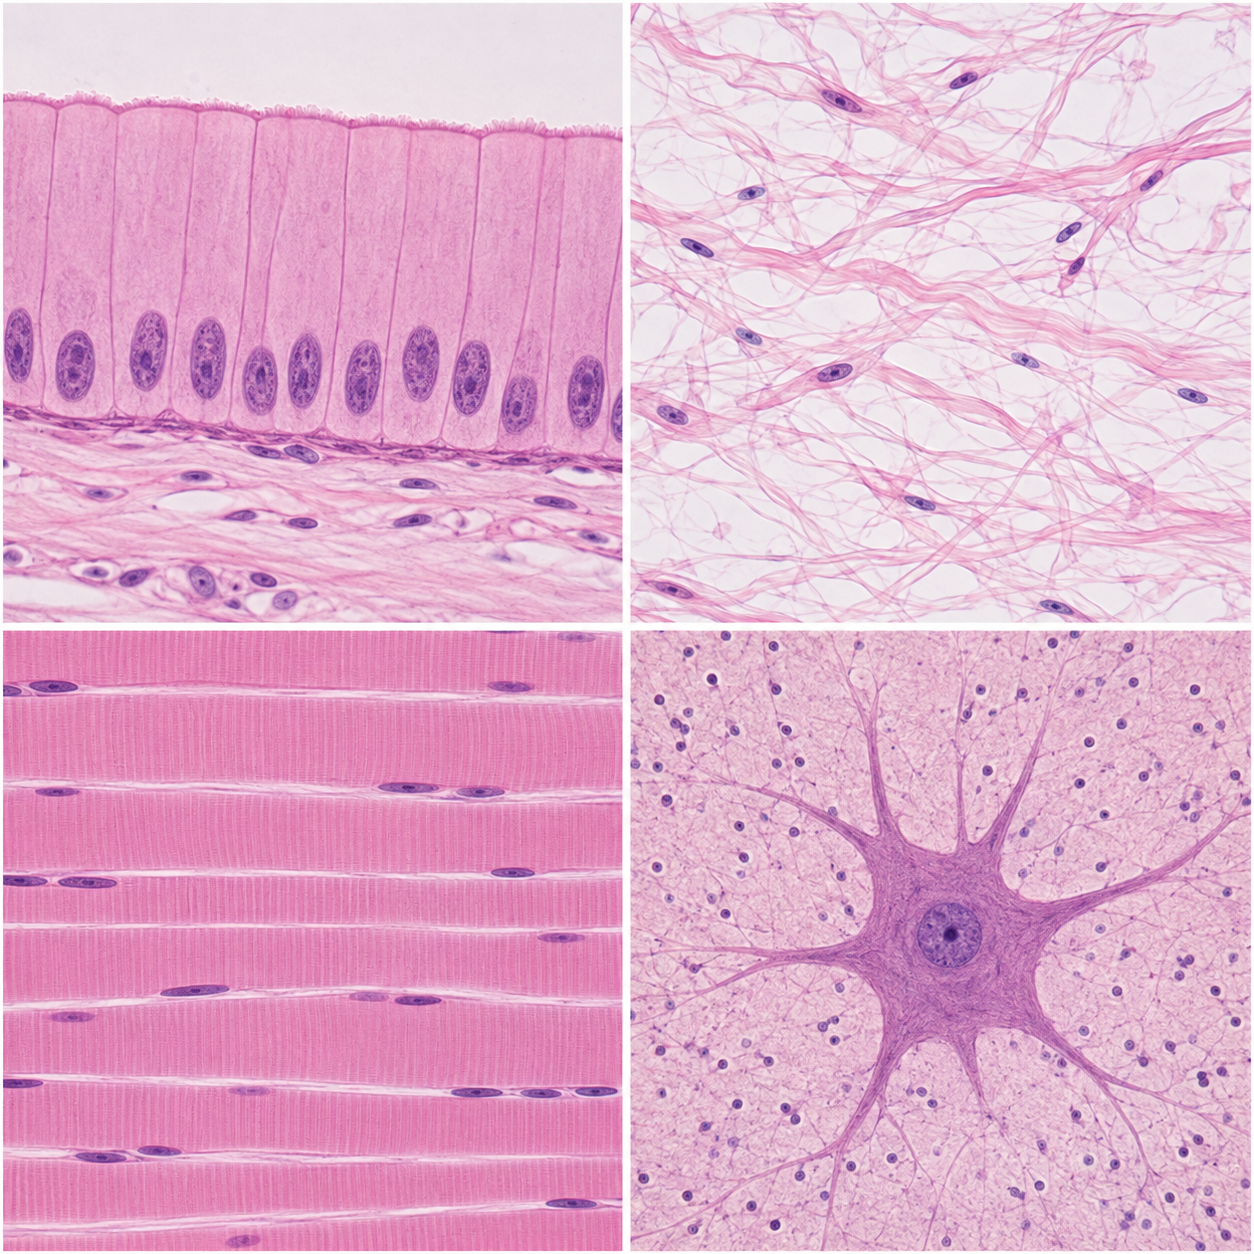
\includegraphics[width=0.6\linewidth]{images/book3/ai/b3-04-tissues.png}

{\small सूक्ष्मदर्शी के नीचे \omterm{def:b1:body-plans-tissues:tissue}{ऊतकों} के चार प्रकार। ऊपर बाएँ: सरल
स्तंभाकार \omterm{def:b1:body-plans-tissues:epithelium}{उपकला}, ऊँची कोशिकाओं की एक ही पंक्ति। ऊपर दाएँ: ढीला \omterm{def:b1:body-plans-tissues:connective}{संयोजी
ऊतक}, लहरदार \omterm{def:b1:body-plans-tissues:connective}{कोलैजन} तंतुओं के बीच बिखरी कोशिकाएँ। नीचे बाएँ: कंकाल पेशी
के तंतु, धारीदार, जिनके किनारों पर केंद्रक हैं। नीचे दाएँ: \omterm{def:b1:body-plans-tissues:nervous}{ग्लियल
कोशिकाओं} के बीच एक \omterm{def:b1:body-plans-tissues:nervous}{न्यूरॉन}।}
\end{omfigure}

\begin{example}[ऊतक कहाँ से आते हैं]\label{ex:b1:body-plans-tissues:origin}
\omterm{def:b1:body-plans-tissues:epithelium}{उपकलाएँ} तीनों जनन स्तरों से निकलती हैं (त्वचा \omterm{def:b1:body-plans-tissues:layers}{बाह्यचर्म} से, आँत का
अस्तर \omterm{def:b1:body-plans-tissues:layers}{अंतश्चर्म} से, वाहिकाओं तथा \omterm{def:b1:body-plans-tissues:layers}{देहगुहा} का अस्तर \omterm{def:b1:body-plans-tissues:layers}{मध्यचर्म} से); \omterm{def:b1:body-plans-tissues:connective}{संयोजी
ऊतक}, पेशी और रक्त \omterm{def:b1:body-plans-tissues:layers}{मध्यचर्म} से; और \omterm{def:b1:body-plans-tissues:nervous}{तंत्रिका ऊतक} \omterm{def:b1:body-plans-tissues:layers}{बाह्यचर्म} से। मेंढक की
त्वचा मध्यचर्मी \omterm{def:b1:body-plans-tissues:connective}{संयोजी ऊतक} पर बैठी एक बाह्यचर्मी \omterm{def:b1:body-plans-tissues:epithelium}{उपकला} है; उसकी आँत
मध्यचर्मी पेशी में लिपटी एक अंतश्चर्मी \omterm{def:b1:body-plans-tissues:epithelium}{उपकला}; और उसका मस्तिष्क भीतर की
ओर मुड़ा \omterm{def:b1:body-plans-tissues:layers}{बाह्यचर्म}।
\end{example}

\section{ऊतकों से एक अंग तक: आँत की भित्ति}

\begin{proposition}[आँत की भित्ति की चार परतें]\label{prop:b1:body-plans-tissues:gutwall}
\index{आँत की भित्ति}
अवकाशिका से बाहर की ओर चलें तो कशेरुकी पाचन नली की भित्ति चार संकेंद्री
परतों से बनी है, और हर परत \omterm{def:b1:body-plans-tissues:tissue}{ऊतकों} का एक संयोजन है: \emph{श्लेष्मिका}
(वाहिकाएँ तथा \omterm{def:b1:mammal-organization:compartments}{लसीका} वाहिकाएँ ढोते किसी ढीले \omterm{def:b1:body-plans-tissues:connective}{संयोजी ऊतक} पर बैठी एक
\omterm{def:b1:body-plans-tissues:epithelium}{उपकला} --- अवशोषक और स्रावी --- जिसके नीचे चिकनी पेशी की एक पतली चादर
है); \emph{अधःश्लेष्मिका} (बड़ी वाहिकाओं और एक तंत्रिका-जाल सहित सघन
\omterm{def:b1:body-plans-tissues:connective}{संयोजी ऊतक}); \emph{पेशीस्तर} (चिकनी पेशी की दो परतें, भीतरी वर्तुल और
बाहरी अनुदैर्घ्य, जिनके बीच एक तंत्रिका-जाल है, और जो मिलाने तथा आगे
ठेलने वाली गतियाँ पैदा करती हैं); और \emph{सीरोसा} (\omterm{def:b1:body-plans-tissues:layers}{देहगुहा} की \omterm{def:b1:body-plans-tissues:epithelium}{उपकला} से
ढकी एक पतली संयोजी परत)। ये चारों परतें ग्रासनली से मलाशय तक चलती हैं;
जो बदलता है वह श्लेष्मिका है --- छोटी आँत में रसांकुरों में मुड़ी हुई,
आमाशय में ग्रंथिल।
\end{proposition}

\begin{omfigure}
\begin{tikzpicture}
  \node[anchor=south west, inner sep=0] (img) at (0,0)
    {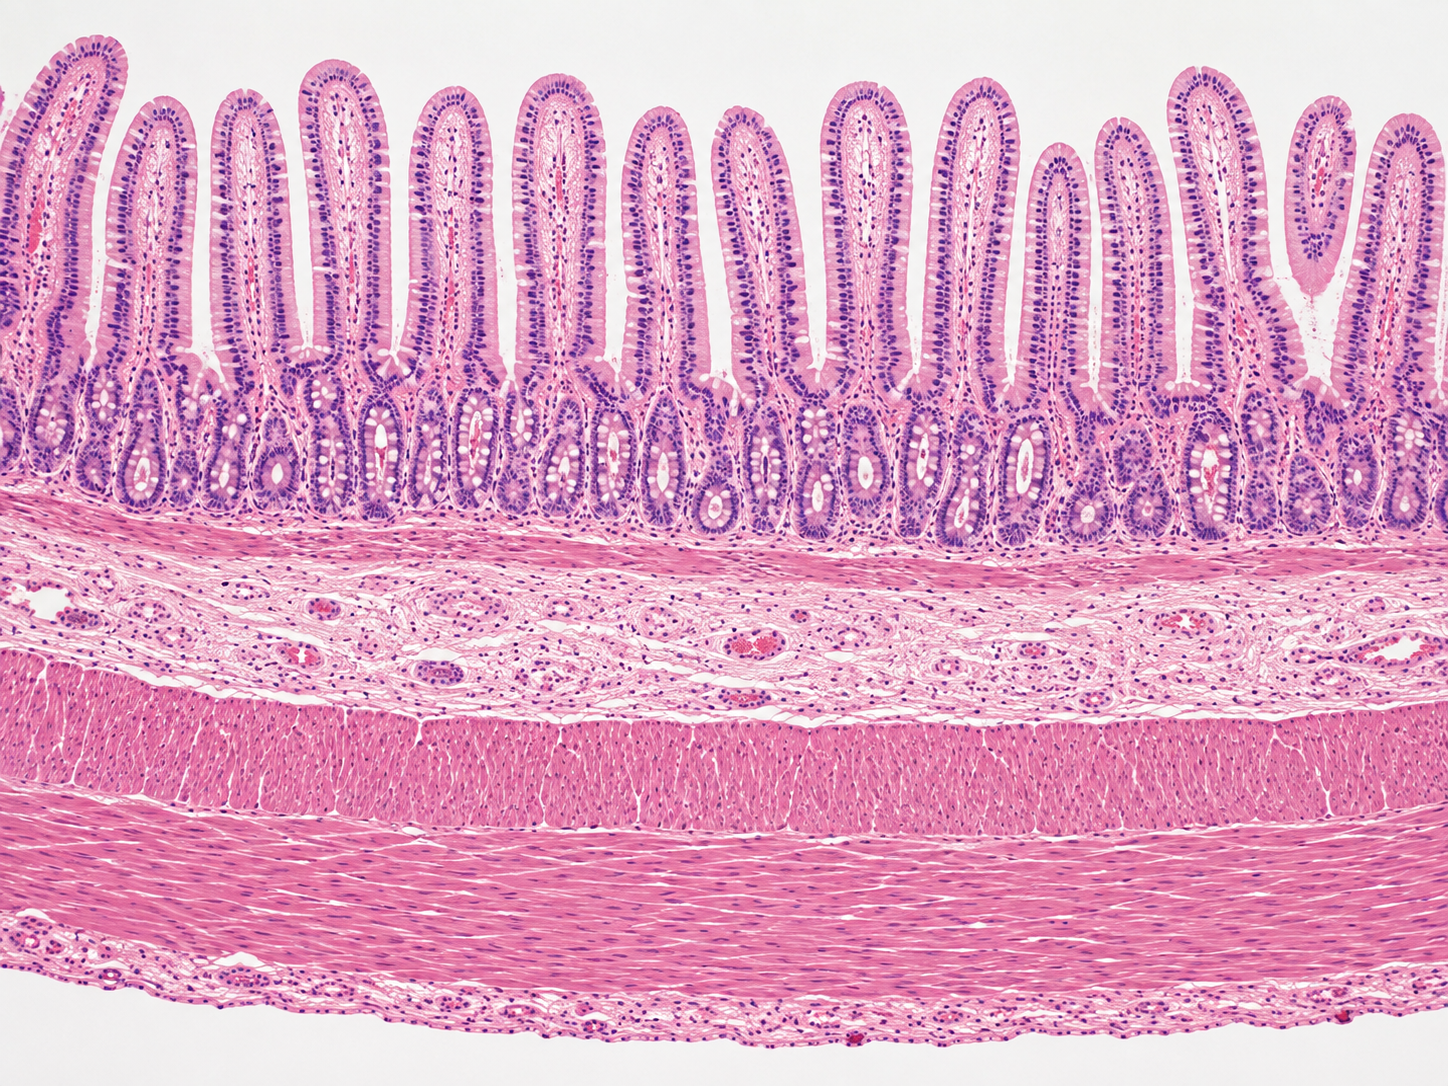
\includegraphics[width=0.53\linewidth]{images/book3/ai/fig-gut-wall-histology.png}};
  \begin{scope}[x={(img.south east)}, y={(img.north west)},
      every node/.style={font=\small}]
    \draw[omDef, thick] (0.50,0.985) -- (0.50,1.08) node[above] {अवकाशिका};
    \draw[omDef, thick] (0.30,0.82) -- (-0.03,0.86) node[left, align=right] {रसांकुर: संयोजी ऊतक\\ पर उपकला};
    \draw[omDef, thick] (0.40,0.58) -- (-0.03,0.56) node[left] {ग्रंथियाँ (गर्तिकाएँ)};
    \draw[omDef, thick] (0.70,0.505) -- (1.03,0.56) node[right] {श्लेष्मिका-पेशीस्तर};
    \draw[omDef, thick] (0.70,0.42) -- (1.03,0.42) node[right] {अधःश्लेष्मिका};
    \draw[omDef, thick] (0.70,0.24) -- (1.03,0.26) node[right, align=left] {पेशीस्तर:\\ वर्तुल, अनुदैर्घ्य};
    \draw[omDef, thick] (0.70,0.06) -- (1.03,0.06) node[right] {सीरोसा};
  \end{scope}
\end{tikzpicture}

{\small छोटी \omterm{prop:b1:body-plans-tissues:gutwall}{आँत की भित्ति} की अनुप्रस्थ काट। श्लेष्मिका के रसांकुर
अवकाशिका में निकले हैं; उनके नीचे ग्रंथियाँ, पेशी की एक पतली चादर,
अधःश्लेष्मिका, पेशीस्तर की दो परतें और सीरोसा। चार परतें, चार \omterm{def:b1:body-plans-tissues:tissue}{ऊतक}
प्रकार, एक \omterm{def:b1:mammal-organization:organ}{अंग}।}
\end{omfigure}

\begin{method}[किसी ऊतकवैज्ञानिक काट को पढ़ना]\label{met:b1:body-plans-tissues:histology}
\begin{enumerate}
  \item मुक्त सतह या अवकाशिका खोजिए: उसे अस्तरित करती \omterm{def:b1:body-plans-tissues:epithelium}{उपकला} ही पहली
        परत है। उसके केंद्रकों की पंक्तियाँ गिनिए (सरल या स्तरित) और
        कोशिकाओं की आकृति देखिए।
  \item \omterm{def:b1:body-plans-tissues:epithelium}{उपकला} के नीचे बिखरे केंद्रकों और वाहिकाओं वाले उस फीके, तंतुमय
        क्षेत्र को खोजिए: वह \omterm{def:b1:body-plans-tissues:connective}{संयोजी ऊतक} है।
  \item पेशी लंबी कोशिकाओं के सघन गुच्छों के रूप में दिखती है:
        परिधीय केंद्रकों सहित धारीदार (कंकाल), धारीदार और शाखित
        (हृदय), केंद्रीय केंद्रक सहित बिना धारी वाली (चिकनी)। काट के
        सापेक्ष तंतुओं की दिशा देखिए।
  \item किसी \omterm{def:b1:mammal-organization:organ}{अंग} की भित्ति में \omterm{def:b1:body-plans-tissues:nervous}{तंत्रिका ऊतक} पेशी परतों के बीच बड़े फीके
        न्यूरॉन-कायों के गुच्छों के रूप में दिखता है।
  \item परतों के क्रम और श्लेष्मिका की विशिष्टताओं (रसांकुर, ग्रंथियाँ,
        केराटिन) से \omterm{def:b1:mammal-organization:organ}{अंग} का नाम बताइए।
\end{enumerate}
\end{method}

\begin{example}[विनिमय सतह के रूप में रसांकुर]\label{ex:b1:body-plans-tissues:villus}
मानव छोटी आँत का एक रसांकुर \qty{0.6}{mm} ऊँची और \qty{0.15}{mm} चौड़ी
एक उँगली है, जो स्तंभाकार कोशिकाओं की एक ही परत से ढकी है और जिनके हर
शीर्ष फलक पर कोई \qty{1500}{} सूक्ष्मांकुर हैं। रसांकुर नली की सतह लगभग
सात गुना कर देते हैं और सूक्ष्मांकुर उसे फिर बीस गुना: सादी नली के
\qty{0.6}{m^2} दसियों वर्ग मीटर अवशोषक \omterm{def:b1:body-plans-tissues:epithelium}{उपकला} बन जाते हैं, जो एक कोशिका
मोटी है और जिसकी हर कोशिका अपने रसांकुर के संयोजी अंतर्भाग में स्थित
किसी केशिका तथा किसी \omterm{def:b1:mammal-organization:compartments}{लसीका} वाहिका से कुछ ही माइक्रोमीटर दूर है
(\cref{ch:b1:digestion-absorption})। यह \omterm{def:b1:body-plans-tissues:epithelium}{उपकला} हर चार दिन में अपने आधार की
ग्रंथियों से नई बनती है: चादर, उसकी संधियाँ और उसकी ध्रुवता लगातार फिर
से बनती रहती हैं।
\end{example}

\begin{remark}[दोनों आदर्श जीवों के ऊतक]\label{rem:b1:body-plans-tissues:plants}
\cref{ch:b1:flowering-plant-organization} के पौधे के तीन \omterm{def:b1:body-plans-tissues:tissue}{ऊतक} तंत्रों का
यहाँ कोई ठीक-ठीक समकक्ष नहीं है। उसकी \omterm{def:b1:flowering-plant-organization:tissues}{अधिचर्म} कार्य में तो \omterm{def:b1:body-plans-tissues:epithelium}{उपकला} है, पर
उसकी कोशिकाएँ भित्तियों से थमी हैं, संधियों से नहीं; उसका \omterm{def:b1:flowering-plant-organization:tissues}{भरण ऊतक} एक ही
साथ संचय, आधार और प्रकाश-संश्लेषी है; और उसके पास न पेशी है न तंत्रिका।
जंतु के चार \omterm{def:b1:body-plans-tissues:tissue}{ऊतक} उस शरीर के औज़ार हैं जो चलता और भाँपता है; पौधे के तीन,
उस शरीर के जो बढ़ता है।
\end{remark}

\section{अभ्यास}

\begin{exercise}[$\star$]\label{exo:b1:body-plans-tissues:1}
अरीय और \omterm{def:b1:body-plans-tissues:symmetry}{द्विपार्श्व सममिति} की परिभाषा दीजिए और हर एक का एक जंतु बताइए।
इनमें से कौन-सी \omterm{def:b1:mammal-organization:bodyplan}{शीर्षीभवन} के साथ चलती है, और क्यों?
\end{exercise}

\begin{exercise}[$\star$]\label{exo:b1:body-plans-tissues:2}
तीनों \omterm{def:b1:body-plans-tissues:layers}{जनन स्तर} बताइए और हर एक से निकला एक \omterm{def:b1:body-plans-tissues:tissue}{ऊतक}।
\end{exercise}

\begin{exercise}[$\star$]\label{exo:b1:body-plans-tissues:3}
\omterm{def:b1:body-plans-tissues:tissue}{ऊतकों} के चारों प्रकार, उनके परिभाषक लक्षण और हर एक का एक कार्य गिनाइए।
\end{exercise}

\begin{exercise}[$\star$]\label{exo:b1:body-plans-tissues:4}
\omterm{def:b1:body-plans-tissues:epithelium}{उपकला} वाले आलेख से शीर्ष से आधार तक चारों संधियाँ बताइए और हर एक का
काम।
\end{exercise}

\begin{exercise}[$\star\star$]\label{exo:b1:body-plans-tissues:5}
किसी जंतु के तीन \omterm{def:b1:body-plans-tissues:layers}{जनन स्तर} हैं, \omterm{def:b1:body-plans-tissues:layers}{मध्यचर्म} से अस्तरित एक \omterm{def:b1:body-plans-tissues:layers}{देहगुहा} है, एक
आरपार आँत है, एक जैसे खंड हैं और कोई कठोर भाग नहीं। उसकी योजना के लक्षण
एक-एक करके दीजिए और उससे मेल खाता एक समूह बताइए।
\end{exercise}

\begin{exercise}[$\star\star$]\label{exo:b1:body-plans-tissues:6}
समझाइए कि केंचुआ अपनी \omterm{def:b1:body-plans-tissues:layers}{देहगुहा} को कंकाल के रूप में लेकर कैसे चलता है, और
इसमें हर खंड की दोनों पेशी परतों की भूमिका बताइए।
\end{exercise}

\begin{exercise}[$\star\star$]\label{exo:b1:body-plans-tissues:7}
क्रेफ़िश के \omterm{def:b1:body-plans-tissues:segments}{बाह्यकंकाल} और मेंढक के \omterm{def:b1:body-plans-tissues:segments}{अंतःकंकाल} की तुलना कीजिए: वृद्धि,
रक्षा, पेशियों का जुड़ाव, और हर एक जो आकार-सीमा लगाता है।
\end{exercise}

\begin{exercise}[$\star\star$]\label{exo:b1:body-plans-tissues:8}
\omterm{def:b1:organism-environment:organism}{जीव} के नियंत्रण में \omterm{prop:b1:organism-environment:surfaces}{विनिमय सतह} बनने के लिए किसी \omterm{def:b1:body-plans-tissues:epithelium}{उपकला} को दृढ़ संधियाँ
क्यों चाहिए? उनके बिना आँत के अवशोषण का क्या होता?
\end{exercise}

\begin{exercise}[$\star\star$]\label{exo:b1:body-plans-tissues:9}
किसी काट में, अवकाशिका से बाहर की ओर, यह दिखता है: रसांकुरों सहित एक सरल
स्तंभाकार \omterm{def:b1:body-plans-tissues:epithelium}{उपकला}, ढीला \omterm{def:b1:body-plans-tissues:connective}{संयोजी ऊतक}, पेशी की एक पतली चादर, सघन \omterm{def:b1:body-plans-tissues:connective}{संयोजी ऊतक},
पेशी की दो मोटी परतें, और एक पतली बाहरी परत। \omterm{def:b1:mammal-organization:organ}{अंग} और हर परत का नाम
बताइए।
\end{exercise}

\begin{exercise}[$\star\star\star$]\label{exo:b1:body-plans-tissues:10}
उपास्थि में रक्त वाहिकाएँ नहीं होतीं और हड्डी में बहुत होती हैं। इसे इस
बात से जोड़िए कि हर एक कैसे पोषित होती है, कितनी तेज़ी से भरती है, और
शरीर में कहाँ काम आती है।
\end{exercise}

\begin{exercise}[$\star\star\star$]\label{exo:b1:body-plans-tissues:11}
कोई दवा आँत की \omterm{def:b1:body-plans-tissues:epithelium}{उपकला} में दृढ़ संधियों का बनना रोक देती है। \omterm{def:b1:body-plans-tissues:epithelium}{उपकलाओं} के
गुणों की सहायता से अवशोषण पर, \omterm{def:b1:organism-environment:milieu}{आंतरिक पर्यावरण} के संघटन पर और संक्रमण पर
उसके प्रभावों की भविष्यवाणी कीजिए।
\end{exercise}

\begin{exercise}[$\star\star\star$]\label{exo:b1:body-plans-tissues:12}
``\omterm{def:b1:mammal-organization:bodyplan}{शरीर-योजना} बंधनों का समुच्चय है, कोई अभिकल्पना नहीं।'' संधिपादों के
निर्मोचन, कीटों के आकार, कशेरुकियों के खंडों और इस अध्याय की सारणी के
अर्थ की सहायता से एक अनुच्छेद में चर्चा कीजिए।
\end{exercise}

\section{समस्या: छोटी आँत की भित्ति}

\begin{problem}[{सप्ताहांत समस्या --- मानव छोटी आँत की एक ऊतकवैज्ञानिक
शृंखला, नली से लेकर सूक्ष्मांकुर तक पढ़ी गई: परतें, रसांकुर, कोशिकाएँ,
संधियाँ और नवीकरण, और अंत में एक ही रसांकुर की अवशोषक सतह}]
\label{pb:b1:body-plans-tissues:1}
मानव छोटी आँत \qty{6}{m} लंबी और भीतर से \qty{3}{cm} व्यास की एक नली
है। उसकी भित्ति की वर्तुल वलियाँ सादी नली की सतह तिगुनी कर देती हैं।
उसकी श्लेष्मिका मुड़ी हुई सतह के प्रति वर्ग मिलीमीटर \qty{25}{} रसांकुर
धारण करती है, और हर रसांकुर \qty{0.6}{mm} ऊँचा तथा \qty{0.15}{mm} व्यास
का एक बेलन है। रसांकुर स्तंभाकार कोशिकाओं से ढके हैं जिनका शीर्ष फलक
\qty{5}{\micro m} भुजा का एक वर्ग है; हर शीर्ष फलक \qty{1500}{}
सूक्ष्मांकुर धारण करता है, जो \qty{1}{\micro m} लंबे और
\qty{0.1}{\micro m} व्यास के बेलन हैं। \omterm{def:b1:body-plans-tissues:epithelium}{उपकला} हर \qty{4}{} दिन में नई बन
जाती है।

\medskip
\noindent\textbf{भाग I --- परतें।}
किसी अनुप्रस्थ काट को सूक्ष्मदर्शी में देखा जाता है।
\begin{enumerate}
  \item भित्ति की चारों परतें अवकाशिका से बाहर की ओर गिनाइए और हर एक
        में मौजूद \omterm{def:b1:body-plans-tissues:tissue}{ऊतक} प्रकार बताइए।
  \item काट में रसांकुर दिखते हैं। यह पाचन नली का कौन-सा भाग है?
        आमाशय की काट में इसकी जगह क्या दिखता?
  \item पेशीस्तर की दोनों पेशी परतों के बीच बड़ी फीकी कोशिकाओं के
        गुच्छे हैं। वे क्या हैं, और वे किसे नियंत्रित करते हैं?
  \item समझाइए कि दोनों पेशी परतें परस्पर लंब दिशाओं में क्यों चलती
        हैं।
\end{enumerate}

\medskip
\noindent\textbf{भाग II --- सतहें।}
\begin{enumerate}[resume]
  \item सादी नली की भीतरी सतह निकालिए।
  \item वर्तुल वलियों के बाद की सतह निकालिए।
  \item एक रसांकुर की पार्श्व सतह निकालिए (बेलन मानकर, सिरा छोड़कर)।
  \item मुड़ी हुई श्लेष्मिका के प्रति वर्ग मिलीमीटर रसांकुर-सतह
        निकालिए, और वह गुणक भी जिससे रसांकुर सतह बढ़ाते हैं।
  \item रसांकुरों के बाद की सतह निकालिए।
  \item एक सूक्ष्मांकुर की और एक कोशिका के \qty{1500}{} सूक्ष्मांकुरों
        की पार्श्व सतह निकालिए।
  \item वह गुणक निकालिए जिससे सूक्ष्मांकुर किसी कोशिका की शीर्ष सतह
        बढ़ाते हैं।
  \item छोटी आँत की कुल अवशोषक सतह निकालिए।
\end{enumerate}

\medskip
\noindent\textbf{भाग III --- कोशिकाएँ।}
\begin{enumerate}[resume]
  \item एक रसांकुर को ढकती \omterm{def:b1:body-plans-tissues:epithelium}{उपकला} कोशिकाओं की संख्या निकालिए।
  \item छोटी आँत में रसांकुरों की संख्या और उन्हें ढकती \omterm{def:b1:body-plans-tissues:epithelium}{उपकला} कोशिकाओं
        की संख्या निकालिए।
  \item \omterm{def:b1:body-plans-tissues:epithelium}{उपकला} हर \qty{4}{} दिन में नई बनती है। प्रतिदिन और प्रति सेकंड
        कितनी कोशिकाएँ अवकाशिका में झड़ती हैं?
  \item प्रतिस्थापी कोशिकाएँ कहाँ बनती हैं, और इससे विभाजित होती
        कोशिकाओं की स्थिति के बारे में अवशोषक कोशिकाओं के सापेक्ष क्या
        पता चलता है?
  \item कोई \omterm{def:b1:body-plans-tissues:epithelium}{उपकला} कोशिका \qty{25}{\micro m} ऊँची है। छोटी आँत में
        \omterm{def:b1:body-plans-tissues:epithelium}{उपकला} का आयतन और उसका द्रव्यमान निकालिए (घनत्व
        \qty{1.05}{g/cm^3})।
\end{enumerate}

\medskip
\noindent\textbf{भाग IV --- संधियाँ, आधात्री और रसांकुर।}
\begin{enumerate}[resume]
  \item हर कोशिका अपने पड़ोसियों से उसके शीर्ष के चारों ओर घूमती एक
        दृढ़ संधि से सील है। प्रति कोशिका दृढ़ संधि की लंबाई और छोटी
        आँत में उसकी कुल लंबाई निकालिए।
  \item समझाइए कि अवकाशिका का कोई पदार्थ रक्त तक केवल दो कोशिका
        झिल्लियाँ पार करके ही क्यों पहुँच सकता है।
  \item रसांकुर का अंतर्भाग ढीला \omterm{def:b1:body-plans-tissues:connective}{संयोजी ऊतक} है जिसमें एक केशिका-जाल और
        एक केंद्रीय \omterm{def:b1:mammal-organization:compartments}{लसीका} वाहिका है। उसमें मौजूद बाह्यकोशिकीय तंतुओं के
        दोनों प्रकार बताइए और वह कोशिका भी जो उन्हें स्रावित करती है।
  \item \omterm{def:b1:body-plans-tissues:epithelium}{उपकला} के और अंतर्भाग के उद्गम-जनन स्तर बताइए।
  \item रसांकुर में चिकनी पेशी की एक लड़ी भी है जो उसे लयबद्ध रूप से
        छोटा करती है। उसका कार्य सुझाइए।
  \item कोई रोग रसांकुरों को चपटा कर देता है (सतह मुड़ी हुई नली की सतह
        पर लौट आती है)। अवशोषक सतह कितने गुणक से घटती है, और उसके क्या
        परिणाम होते हैं?
  \item एक रसांकुर की, उसके सूक्ष्मांकुरों सहित, अवशोषक सतह वर्ग
        मिलीमीटर में निकालिए।
  \item परिणाम बताइए: एक ही रसांकुर की अवशोषक सतह, और छोटी आँत में
        रसांकुरों की संख्या।
\end{enumerate}
\end{problem}
